\documentclass[11pt]{article}
\usepackage{comment} % enables the use of multi-line comments (\ifx \fi) 
\usepackage{lipsum} %This package just generates Lorem Ipsum filler text. 
\usepackage{fullpage} % changes the margin
\usepackage{graphicx} % Required to insert images
\usepackage{amsmath}
\usepackage{algorithm}
\usepackage{caption}
\usepackage[noend]{algpseudocode}

\makeatletter
\def\BState{\State\hskip-\ALG@thistlm}
\makeatother

\usepackage[hidelinks]{hyperref}
\setlength{\parindent}{0in}

\graphicspath{{./figs/}}
%\urlstyle{same}
%--Title
%\title{ \textbf{STAT 545 Final Project Proposal}%	\small{Due\ on\ Oct 22 2017}\\
%}
%
%\author{\textbf{Jingjing Guo }}
%\date{Oct 22 2017}

%----------------------------------------------------------------------------------------
%	TITLE PAGE
%----------------------------------------------------------------------------------------

%\title{
%	\vspace{.5in}
%	\textbf{STAT 545 Intro to Computational Statistics}\\
%%	\normalsize\vspace{0.1in}\small{Due\ on\ Oct 22, 2017}\\
%	%\vspace{0.1in}\large{\textit{\hmwkClassInstructor\ \hmwkClassTime}}
%	\textbf{Final Project Proposal:} \\ 
%	\vspace{1.5in} 
%	\textbf{Boosting Method in the Sentiment Analysis of Amazon Fine Food Reviews}
%	\vspace{.5in}
%}


\title{
	\vspace{2in}
	\textbf{STAT 545: Final Project Report}\\
	%	\normalsize\vspace{0.1in}\small{Due\ on\ Oct 22, 2017}\\
	%\vspace{0.1in}\large{\textit{\hmwkClassInstructor\ \hmwkClassTime}}
	\vspace{4in} 
%	\textbf{Boosting Method in the Sentiment Analysis of Amazon Fine Food Reviews}
}

\author{\textbf{Jingjing Guo} \\In Collaboration with Yue Zhou}
\date{Dec 15, 2017} % Insert date here if you want it to appear below your name


\begin{document}
%--Title---
\begin{titlepage}
	\maketitle
	\thispagestyle{empty}
\end{titlepage}

\tableofcontents
\newpage

%--Sections---
\section{Problem Overview}
In this project, we conducted a sentiment study of an Amazon fine food review dataset from \href{https://www.kaggle.com/snap/amazon-fine-food-reviews}{Kaggle}. The dataset consists of 568,454 food reviews Amazon users left up to October 2012\cite{rf1}. TheseCloud reviews consist of textual data written by amazon users to express either positive or negative feedback to various products.  An word cloud is shown in Figure \ref{wordCloud} to illustrate contents of the review. \\

\begin{minipage}{\textwidth}		
	\begin{figure}[H]
		\centering
		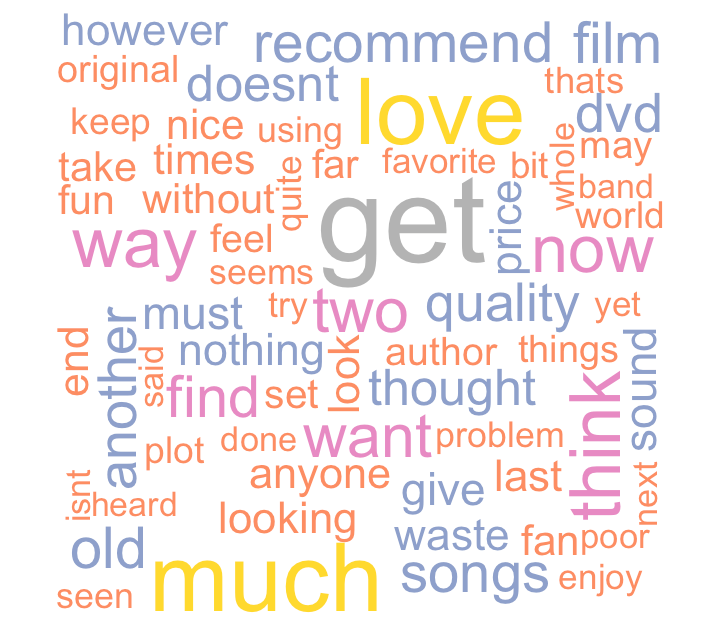
\includegraphics[width=0.5\textwidth]{wc}
		\caption{Word Cloud of the Review Dataset}
		\label{wordCloud}
	\end{figure}
\end{minipage} \hfill

The objective of this project is two fold. First, implementing the random forest model in R. Secondly, use this method to develop a predictive classifier of the review data as positive or negative.\\
\section{Overview of Random Forest}
Random forests are an ensemble learning method for classification and other tasks. It uses a multitude of decision trees for training and learning and outputting the class that based on the statistical results from all decision trees. Random decision forests more effectively explores the model space than a single decision tree and therefore can overcome the over fitting issue of a decision tree, and reduces variance of the prediction.\\

\subsection{Decision Trees}
Decision tree is a simple and widely used method for classification. In the learning or training process, decision tree is built by recursively select the best feature as its node attribute. We use the CART algorithm which uses a Gini-index as its evaluation criterion.\\ Given the training set S, the target attribute (positive review or negative review), Gini index of S is defined as:
$$Gini(S) = 1 - \Sigma_{x} p_i^2$$

And the Gini Gain splitting S by the value of feature A is:
$$Gini(S, A) = Entropy(S) - \Sigma_{v \in values(A)} \frac{|S_A|}{|A|} Entropy(S_A)$$
where,
$$ H(X) = - \sum_x p(x) log_2p(x) $$
This given us how much uncertain we reduced by splitting the data according to feature A.

The model space of a decision tree includes both its structure and attributes at each node. In the learning process, decision trees can be developed by selecting the best attributes with minimal Gini gain and recursively grow until a predetermined constraint is met.\\

In the prediction with new data, each data point will route according to the node attributes of the tree and their corresponding values. The leaf value at the end of the route specifies the classification of the new data.\\
%
%How to split the data is decided by algorithms like information gain, chi square and gini gain. Information gain measures how much the entropy decrease by the classification. Gini gain measures the decrease of Gini index. Chi square calculates the normalized squared deviation of observed (predicted) values from actual values. Here we use the gini index because the other two methods are more computationally expensive. 
%
%Given the training set S, the target attribute (positive review or negative review), Gini index of S is defined as:
%Gini(S)=1-∑_x_p_i^2 
%where p_i is the probability that S belongs to class i. In the code, we write this in gini_index function. We split the data according to one feature and all review with the feature value equals to 1 belongs to one part and the feature value equals to 0 belongs to another.
%
%Gini_gain function is to evaluation criterion for selecting feature A which is define as:
%Gain(S,A)=Gini(S)-∑_(v∈valve(A))▒|S_i |/|S|  Gini(S_i)
%where S_i is the partition of S is induced by the value of feature A. This given us how much uncertain we reduced by splitting the data according to feature A.

\subsection{Bootstrap Aggregation}
Random forests are a variant that aims to improve on bagged Decision Trees by reducing the correlation between the models. First, each tree is learned from a bootstrap sample, and second for each tree split, a random sample of k features is drawn first, and only those features are considered when selecting the best feature to split on (typically $k=\sqrt{p}$ or $k=log p$).\\

 A single tree is highly sensitive to noise in its training. The essential idea in bagging is to average many noisy but approximately unbiased models, and hence reduce the variance \cite{rf2}.\\

\section{Implementation}
\subsection{Data Pre-processing}
The reviews are in a FastText Form with labels 1 or 2, with 1 being one-star or 2-star review and 2 being 4-star or 5-star review. An example of the data is shown in Figure \ref{reviewExample}.\\

To process these textual data, we first select m top most common words for all entries in dataset as features. Each entry is then converted into vectors of 0 or 1, with the 1 representing the entry containing the i-th feature word, and 0 otherwise. This way, we are able to generate a matrix of size $(m+1) \times n$ and elements of 0 or 1.\\

\begin{minipage}{\textwidth}		
	\begin{figure}[H]
		\centering
		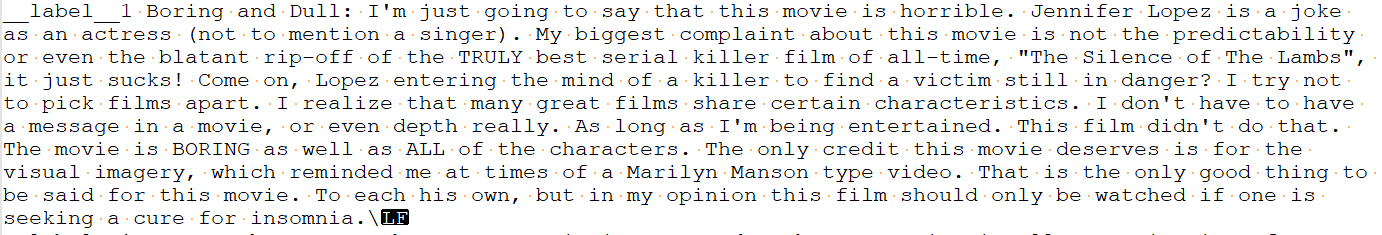
\includegraphics[width=0.95\textwidth]{reviewExample}
		\caption{Review Example}
		\label{reviewExample}
	\end{figure}
\end{minipage} \hfill

\subsection{Algorithms}
\textbf{Decision Tree} Pseudo code for the algorithm we implement for decision tree is shown in Algorithm \ref{dt}. 
Note in this algorithm, we specify depth of the tree and minimal size of data for leaves (bottom level nodes) as constraints. The more detailed code are appended to this report. \\

A nested list is used for storing the tree structure and attributes of each node. At each level, a node is represented with three attributes: index, left and right, where left or right themselves are may be lists of the same data structure as well.\\


\begin{algorithm}[H]
	\caption{Decision Tree}\label{dt}
	\begin{algorithmic}[1]
		\State $Root \gets \textit{Divide data once with best feature}$
		\Procedure{Build Tree}{}
		\State $\text{Intialize variable to store tree attributes, e.g. a nested list, tree}$
		\If {$\textit{splitted table is pure}$} 
		\State $tree_{left} = toLeaf(data_{left} + data_{right} )$  
		\State $tree_{right} = toLeaf(data_{left} + data_{right} )$  \Return
		\EndIf
		
		\If {$\textit{Tree Level} >= Maximum Level$} 
		\State $tree_{left} = toLeaf(data_{left})$  
		\State $tree_{right} = toLeaf(data_{right})$
		\Return
		\EndIf
		
		\If {$\textit{Left Data Size} <= Mininum Size$} 
		\State $tree_{left} = toLeaf(data_{left})$  
		\Else 
		\State $\textit{Left Data Size} <= Mininum Size$
		\State $\textit{Recurse}$
		\EndIf
		
		\If {$\textit{Right Data Size} <= Mininum Size$} 
		\State $tree_{right} = toLeaf(data_{right})$  
		\Else 
		\State $\textit{right Data Size} <= Mininum Size$
		\State $\textit{Recurse}$
		\EndIf
		\EndProcedure
		\State $Root \gets Build Tree(Root, Maximum_Lvel, Min_Size, 1)$
	\end{algorithmic}
\end{algorithm}

\textbf{Random Forest}: The random forest algorithm use decision tree procedure, and randomly selected k features to create $p$ trees. 


\begin{algorithm}[H]
	\caption{Random Forest}\label{rf}
	\begin{algorithmic}[2]
		\State $k \gets \sqrt{m_{features}}$
		
		\Procedure{Random Forest}{}
		\State $\text{Initialize variable to store trees}$
		
		
		\For {$i \in \text{1 to number of trees}$}
		\State $\text{Sample k features from m features}$ 
		\State $\text{Recreate Training Data}$ 
		\State $\text{Use new Training data to build a new tree}$
		\State $\text{Attach tree to Trees}$
		\EndFor
		
		\EndProcedure
	\end{algorithmic}
\end{algorithm}


\section{Results and Analysis}
In studying the model, we varied four parameters: training data size, number of features, number of trees and maximal depth of tree. The results are shown in Figures \ref{res} a)-d). The values of other variables are listed in Table \ref{tab1}. In all cases, we use 1000 examples for testing, and each case is run 10 times to estimate model variance. The test datasets are new data that do not overlap with the training data.\\
\begin{table}[H]
	\caption{Parameter Setting for Implementation Cases}
	\label{tab1}s
	\begin{tabular}{|c |c |c |c |c|}
		\hline
		Figure Index & Training Data Size & Number of Features & Number of Trees & Maximum Depth\\
		\hline
		\ref{res}-a) & Varying & 1000 & 50 & 15 \\
		\hline
		\ref{res}-b) & 5000 & Varying & 50 & 15 \\
		\hline
		\ref{res}-c) & 5000 & 1000 & Varying & 15\\
		\hline
		\ref{res}-d) & 5000 & 1000 & 50 & Varying \\
		\hline
	\end{tabular}
\end{table}

The performance metric we use to evaluate each model is prediction error rate, i.e. the percentage of erroneous prediction for the new dataset.\\

\begin{table}[H]
	\begin{tabular}{c c}
		\begin{minipage}{.45\textwidth}
			\centering		
			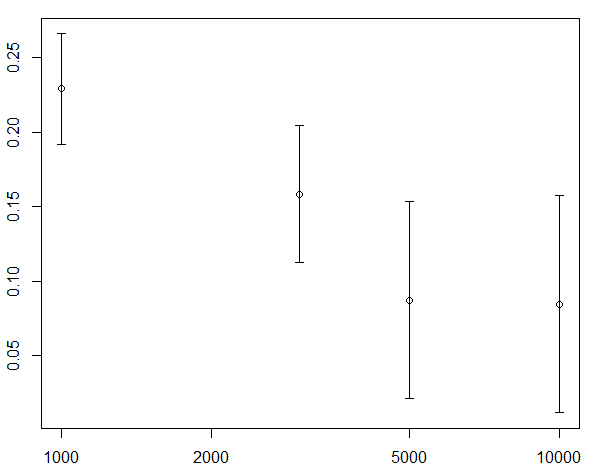
\includegraphics[width=0.99\textwidth]{ts}
		\end{minipage}
		&
		\begin{minipage}{.45\textwidth}
			\centering
			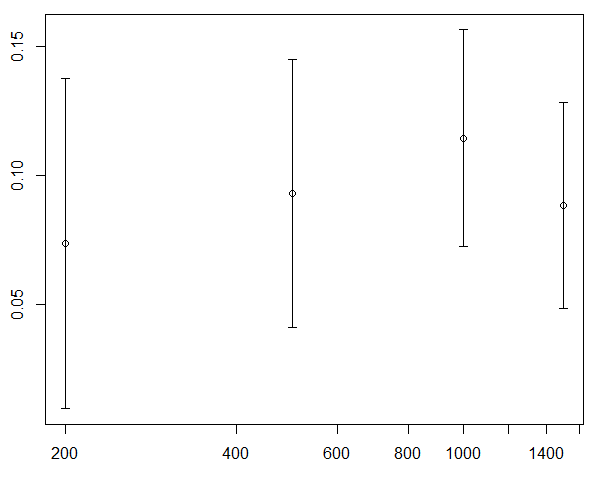
\includegraphics[width=0.99\textwidth]{nf}
		\end{minipage} 
		\\
		a) Training Size & b) Number of Features\\
		\begin{minipage}{.45\textwidth}
			\centering
			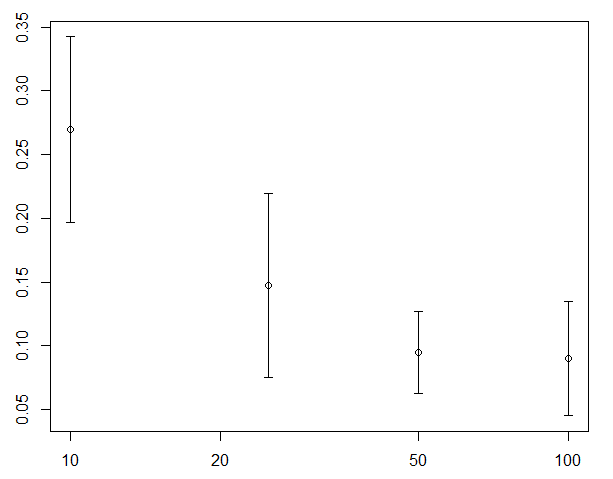
\includegraphics[width=0.99\textwidth]{nt}
		\end{minipage} 
		&
		\begin{minipage}{.45\textwidth}
			\centering
			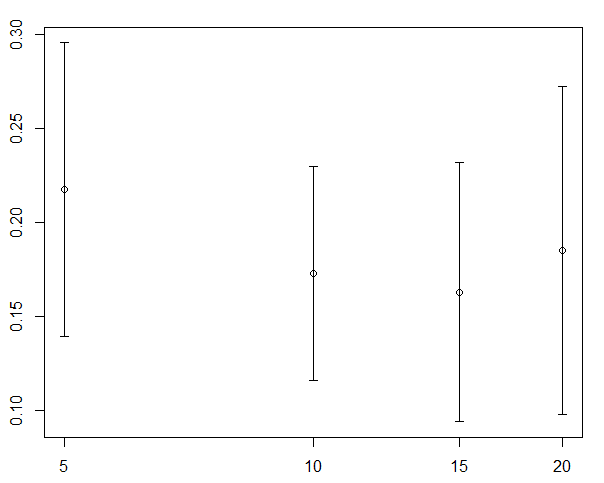
\includegraphics[width=0.99\textwidth]{md}
		\end{minipage} \\
		c) Number of Trees & d) Maximal Depth
	\end{tabular} \hfill
	\captionof{figure}{\small Plots of Prediction Error Rate for Varying Training Size, Number of Features, Number of Trees and Max Depth}
	\label{res}
\end{table}

From this result, we can see that with the increase of training size, the error rate decreases as expected. This is because larger data contains more information about the generative model and the trained model better approximate the true model and thus the prediction error rate for the new data set will decrease.\\

For the number of features, the performance did not seem to improve as the number of features increase, this is likely due to the fixed value of k which randomly selects k features from the m total of features and thus the feature space for the individual decision tree remain the same size. Normally, as the feature space increase, accuracy of the model should also increase. It is possible this is an implementation error in the random forest.\\

For the number of trees, as the number of trees increase, the trained model also seem to be more accurate. The decreasing rate however plateaus eventually. With the dataset size of 5000, this implies inadequacy of data with models that have larger model space. Comparing the cases when the number of trees is 50 and the number of trees is 100, the results show higher variance for 100 trees.\\

For the maximal tree depth of varying values, we also see an initial decrease of prediction error, but the value increases after 15 levels. The variance for 15 and 20 levels also seems excessive. This can also be due to over-fitting. It would be interesting to use a larger training dataset and examine the variance for these depth settings.\\

\subsection{Reflection and Concluding Remarks}
For this project, we intended to study and implement Random Forest models to an Amazon food review dataset for sentiment analysis. We were able to complete the implementation in R and develop random forest models. The original plan was to use most or all of the 500 MB data for training the model. Due to limited resources and extended implementation time, we were unable to accomplish the second objective. \\

We instead sampled about 10K entries of reviews and used that to explore the performance of the method. As was discussed in the preceding section, we looked at varying training sizes, feature sizes, number of trees, and levels of trees for the sampled data. Some of the trends are as expected, but we also observed trends I believe are inconsistent with characteristics of the random forest model, e.g. increased variance with lager model space, and decreased performance with increased number of features. \\

There are a few challenges I want to highlight. First, both team members are new to the R programming language and therefore, some unexpected features of the language, e.g. matrix assignment and manipulations introduced code errors and took us a long time to debug. Second, limited computing power: processing the original dataset exceeded both team member's laptop computing powers, and we were not able to find alternative solutions within the time frame of this project. Finally, there are some theories of random forest models that yet to be studied in depth, the results and analysis in Section 4 require further experiments and explanations.\\

Finally, through this process, I learned to implement the random forest model in R and develop predictive models for textual datasets such as online reviews. I also learned numerically how the tree depth, number of trees, etc. affect the performance of such models. 

\begin{thebibliography}{9}
\bibitem{rf1} Andy Liaw, and Matthew Wiener. \emph{Classification and regression by random forest}. R News.
\bibitem{rf2} J. McAuley and J. Leskovec. 2013. \emph{From amateurs to connoisseurs: modeling the evolution of user expertise through online reviews}
\bibitem{rf3} Polikar, R., \emph{Ensemble based systems in decision making}. IEEE Circuits and Systems Magazine, 2006. 6(3).
\bibitem{rf4} Friedman, T.H.R.T.J, \emph{he Elements of Statistical Learning}. 2008.

\end{thebibliography}

\end{document}
